\def\year{2017}\relax
%File: formatting-instruction.tex
\documentclass[letterpaper]{article} %DO NOT CHANGE THIS
\usepackage{aaai18}  %Required
\usepackage{times}  %Required
\usepackage{helvet}  %Required
\usepackage{courier}  %Required
\usepackage{url}  %Required
\usepackage{graphicx}  %Required
\frenchspacing  %Required
\setlength{\pdfpagewidth}{8.5in}  %Required
\setlength{\pdfpageheight}{11in}  %Required
%PDF Info Is Required:
  \pdfinfo{}
\setcounter{secnumdepth}{0}

\usepackage{amsmath}
\usepackage{amssymb}
\usepackage{amsthm}
\usepackage{multirow}
\usepackage{tikz}
\usepackage{comment}

\usepackage{graphicx}
\usepackage{caption}
\usepackage{subcaption}
\usepackage{listings}
\usepackage{multicol}
\usepackage{arydshln}
\usetikzlibrary{calc,backgrounds,positioning,fit}


\newcommand{\tup}[1]{{\langle #1 \rangle}}

\newcommand{\pre}{\mathsf{pre}}     % precondition
\newcommand{\del}{\mathsf{del}}     % effect
\newcommand{\add}{\mathsf{add}}     % effect
\newcommand{\eff}{\mathsf{eff}}     % effect
\newcommand{\cond}{\mathsf{cond}}   % conditional effect
\newcommand{\true}{\mathsf{true}}   % true
\newcommand{\false}{\mathsf{false}} % false
\newcommand{\PE}{\mathrm{PE}}     % precondition
\newcommand{\strips}{\textsc{Strips}}     % precondition

\newtheorem{theorem}{Theorem}
\newtheorem{lemma}[theorem]{Lemma}
\newtheorem{definition}[theorem]{Definition}


\begin{document}

\title{Learning STRIPS action models with classical planning}

\author{Diego Aineto\and Sergio Jim\'enez\and Eva Onaindia\\
{\small Departamento de Sistemas Inform\'aticos y Computaci\'on}\\
{\small Universitat Polit\'ecnica de Val\'encia.}\\
{\small Camino de Vera s/n. 46022 Valencia, Spain}\\
{\small \{dieaigar,serjice,onaindia\}@dsic.upv.es}}
 
\maketitle
\begin{abstract}
This paper presents a novel approach for learning STRIPS action models from examples that compiles this particular inductive learning task into a classical planning task. Interestingly, the compilation approach is flexible to different amounts of available input knowledge; the learning examples can range from a set of plans (with their corresponding initial and final states) to just a set of initial and final states where neither actions nor intermediate states are given. What is more, the compilation accepts partially specified action models can also be used to validate whether certain observations of plan executions follow a given STRIPS action model (even if the action model is not fully specified).
\end{abstract}


\section{Introduction}
Besides {\em plan synthesis}~\cite{ghallab2004automated,geffner:book:2013}, planning action models are also useful for {\em plan/goal recognition}~\cite{ramirez2012plan}. At both planning tasks, an automated planner is required to reason about action models that correctly and completely capture the possible world transitions. Unfortunately, building planning action models is complex, even for planning experts, and this knowledge acquisition task is a bottleneck that limits the potential of automated planning~\cite{kambhampati:modellite:AAAI2007}.  

On the other hand, Machine Learning (ML) has shown to be able to compute a wide range of different kinds of models from examples~\cite{michalski2013machine}. The application of inductive ML to the learning of STRIPS action models, the vanilla action model for planning~\cite{fikes1971strips}, is not straightforward though:
\begin{itemize}
\item The inputs to ML algorithms (the learning data) usually are finite vectors that encode the value of fixed features for a given set of objects. The input for learning planning action models are observations of plan executions (where each plan possibly has a different length).
\item The traditional output of ML algorithms is a scalar value (an integer, in the case of classification tasks, or a real value, in the case of regression tasks). When learning STRIPS action models the output is, for each action, the sets of preconditions, negative and positive effects, that define the possible state transitions of the corresponding planning domain. 
\end{itemize}

The learning of STRIPS action models is a well-studied problem with sophisticated algorithms, like {\sc ARMS}~\cite{yang2007learning}, {\sc SLAF}~\cite{amir:alearning:JAIR08} or {\sc LOCM}~\cite{cresswell2013acquiring} that do not require full knowledge of the intermediate states traversed by the example plans. Motivated by recent advances on learning different kinds of generative models with classical planning~\cite{bonet2009automatic,segovia2016hierarchical,segovia2017generating}, this paper introduces an innovative approach for learning STRIPS action models that can be defined as a classical planning compilation so an off-the-shelf planner can be used to address the learning task. The compilation approach is appealing because it opens the door to the bootstrapping of planning action models but also because:
\begin{enumerate}
\item Is flexible to different amounts of available input knowledge. The learning examples can range from a set of plans (with their corresponding initial and final states) to just a set of initial and final states where no intermediate actions or states are observed.
\item Accepts previous knowledge about the structure of the actions in the form of partially specified action models. In the extreme, the compilation can be used to validate whether observed plan executions are valid for a given STRIPS action model.
\end{enumerate}

The paper is organized as follows. The first section presents the classical planning model, its extension to conditional effects (which is a requirement of the proposed compilation) and formalizes the STRIPS action model (the output of the addressed learning task). The second section formalizes the learning of STRIPS action models with regard to different amounts of input knowledge. The third and foruth sections describe our approach for addressing this particular learning task by compiling it into classical planning and how previous knowledge can be introduced in the compilation to reduce the space of possible action models and making learning more practicable. Finally the last sections report the data collected during the empirical evaluation of our approach, discusses the strengths and weaknesses of our approach and proposes several opportunities for future research. 
 

\section{Background}
This section defines the planning models used on this work as well as the STRIPS action model, the output of the learning task addressed in this paper.

\subsection{Classical planning}
We use $F$ to denote the set of {\em fluents} (propositional variables) describing a state. A {\em literal} $l$ is a valuation of a fluent $f\in F$, i.e. either~$l=f$ or $l=\neg f$. A set of literals $L$ represents a partial assignment of values to fluents (WLOG we assume that $L$ does not assign conflicting values to any fluent) and let $\neg L=\{\neg l:l\in L\}$ be the complement of $L$. We use $\mathcal{L}(F)$ to denote the set of all literal sets on $F$, i.e.~all partial assignments of values to fluents.

A {\em state} $s$ is then a total assignment of values to fluents, i.e. $|s|=|F|$, so the size of the state space is $2^{|F|}$. Explicitly including negative literals $\neg f$ in states simplifies subsequent definitions but often, we abuse notation by defining a state $s$ only in terms of the fluents that are true in $s$, as is common in \strips\ planning.

A {\em classical planning frame} is a tuple $\Phi=\tup{F,A}$, where $F$ is a set of fluents and $A$ is a set of actions. Each action $a\in A$ has a set of literals $\pre(a)\in\mathcal{L}(F)$, called {\em preconditions}, a set of effects $\eff(a)\in\mathcal{L}(F)$. An action $a\in A$ is {\em applicable} in state $s$ iff $\pre(a)\subseteq s$, and the result of applying $a$ in $s$ is the {\em succesor} state $\theta(s,a)=(s\setminus \neg\eff(a))\cup\eff(a)$.

A {\em classical planning problem} is a tuple $P=\tup{F,A,I,G}$, where $I$ is an initial state and $G\in\mathcal{L}(F)$ is a goal condition. A {\em plan} for $P$ is an action sequence $\pi=\tup{a_1, \ldots, a_n}$ that induces a state sequence $\tup{s_0, s_1, \ldots, s_n}$ such that $s_0=I$ and, for each {\small $1\leq i\leq n$}, $a_i$ is applicable in $s_{i-1}$ and generates the successor state $s_i=\theta(s_{i-1},a_i)$. A plan $\pi$ {\em solves} $P$ iff $G\subseteq s_n$, i.e.~if the goal condition is satisfied at the last state reached after following the application of $\pi$ in $I$.


\subsection{Classical planning with conditional effects}
Our approach for leaning STRIPS action models is compiling this leaning task into a classical planning task with conditional effects. Conditional effects allow us to compactly define actions whose particular effects depend on the current state. Nowadays many classical planners cope with conditional effects without compiling them away. In fact, the support of conditional effects was a requirement for participating at the IPC-2014~\cite{vallati:IPC:AIM2015} and IPC-2018.

Now an action $a\in A$ has a set of literals $\pre(a)\in\mathcal{L}(F)$ called the {\em precondition} and a set of conditional effects $\cond(a)$. Each conditional effect $C\rhd E\in\cond(a)$ is composed of two sets of literals $C\in\mathcal{L}(F)$ (the condition) and $E\in\mathcal{L}(F)$ (the effect).

An action $a\in A$ is {\em applicable} in state $s$ if and only if $\pre(a)\subseteq s$, and the resulting set of {\em triggered effects} is
\[
\eff(s,a)=\bigcup_{C\rhd E\in\cond(a),C\subseteq s} E,
\]
i.e.~effects whose conditions hold in $s$. The result of applying $a$ in $s$ is the {\em succesor} state $\theta(s,a)=(s\setminus \neg \eff(s,a))\cup\eff(s,a)$.


\subsection{The STRIPS action model}
This work addresses the learning of action schemes defined in the STRIPS language~\cite{fikes1971strips}. To formalized the output of this learning task, we assume that there exists a set of {\em predicates} $\Psi$ and that the fluents in $F$ are instantiated from these predicates, as in PDDL~\cite{mcdermott1998pddl,fox2003pddl2}.

Formally, each predicate $p\in\Psi$ has an argument list of arity $ar(p)$. Given a set of objects $\Omega$, the set of fluents $F$ is then induced by assigning objects in $\Omega$ to the arguments of predicates in $\Psi$, i.e.~$F=\{p(\omega):p\in\Psi,\omega\in\Omega^{ar(p)}\}$ s.t. $\Omega^k$ is the $k$-th Cartesian power of $\Omega$.

Likewise, we assume that actions are instantiated from STRIPS operator schemes. Figure~\ref{fig:stack} shows the STRIPS operator schema that corresponds to the {\em stack} action from the blocksworld~\cite{slaney2001blocks} represented in PDDL.
\begin{figure}[hbt]
\begin{footnotesize}
\begin{verbatim}
(:action stack
  :parameters (?x1 ?x2 - object)
  :precondition (and (holding ?x1) 
                     (clear ?x2))
  :effect (and (not (holding ?x1)) 
               (not (clear ?x2))
               (clear ?x1) 
               (handempty) 
               (on ?x1 ?x2)))
\end{verbatim}
\end{footnotesize}
 \caption{\small Example of a STRIPS operator schema that corresponds to the {\em stack} action from the blocksworld represented in PDDL.}
\label{fig:stack}
\end{figure}

Let $\Omega_v$ be a new set of objects, $\Omega\cap\Omega_v=\emptyset$, that represents {\em variable names} and whose cardinality, $|\Omega_v|$, is given by the maximum arity of an action in a given planning frame $\Phi$. For instance, in a three-block blocksworld $\Omega=\{block_1, block_2, block_3\}$ while $\Omega_v=\{v_1, v_2\}$ because operators {\small\tt stack} and {\small\tt unstack}, the ones with the maximum arity, have two parameters.

Let us define also a new set of fluents $F_{v}$ that results instantiating $\Psi$ but using only the {\em variable objects} in $\Omega_v$. In the blocksworld $F_v$={\small\tt\{handempty, holding($v_1$), holding($v_2$), clear($v_1$), clear($v_2$), ontable($v_1$), ontable($v_2$), on($v_1,v_1$),on($v_1,v_2$), on($v_2,v_1$),on($v_2,v_2$)\}}.

We are now ready to define a STRIPS action model $\Xi$ as a set of operator schema $\xi=\tup{head(\xi),pre(\xi),add(\xi),del(\xi)}$ such that:
\begin{itemize}
\item $head(\xi)=\tup{name(\xi),pars(\xi)}$, is the operator {\em header} defined by its corresponding action name and a enumeration of the variable names whose cardinality is the operator arity, $pars(\xi)\in\Omega_v^{ar(\xi)}$. The headers for a 4-operator blocksworld are {\small\tt pickup($v_1$), putdown($v_1$), stack($v_1,v_2$)} and {\small\tt unstack($v_1,v_2$)}.
\item The preconditions $pre(\xi)\subseteq F_v$, the negative effects $del(\xi)\subseteq F_v$, and the positive effects $add(\xi)\subseteq F_v$ such that, $del(\xi)\subseteq pre(\xi)$, $del(\xi)\cap add(\xi)=\emptyset$ and $pre(\xi)\cap add(\xi)=\emptyset$.
\end{itemize}


\section{Learning STRIPS action models}
Learning STRIPS action models from fully available input knowledge, i.e. from plans where the {\em pre-} and {\em post-states} of every action in a plan are available, is straightforward. In this case, a STRIPS operator schema is derived by lifting the literals that change between the pre and post-state of the corresponding action executions. Likewise, the preconditions are derived lifting the minimal set of literals that appears in all the pre-states that correspond to the same operator schema.

This section formalizes more challenging learning tasks, where less input knowledge is available.

\subsection{Learning from labeled plans}
This learning task is formalized as $\Lambda=\tup{\Psi,\Pi,\Sigma}$: 
\begin{itemize}
\item $\Psi$, the set of predicates that define the abstract state space of a given planning domain. 
\item $\Pi=\{\pi_1,\ldots,\pi_{\tau}\}$, the given set of example plans s.t. each plan $\pi_t=\tup{a_1^t, \ldots, a_n^t}$, {\small $1\leq t\leq \tau$}, is an action sequence that induces the corresponding state sequence $\tup{s_0^t, s_1^t, \ldots, s_n^t}$ such that, for each {\small $1\leq i\leq n$}, $a_i^t$ is applicable in the state $s_{i-1}^t$ and generates the successor state $s_i^t=\theta(s_{i-1}^t,a_i^t)$.
\item $\Sigma=\{\sigma_1,,\ldots,\sigma_{\tau}\}$, is a set of labels s.t. each plan $\pi_t$, {\small $1\leq t\leq \tau$}, has an associated label $\sigma_t=(s_0^t,s_{n}^t)$ where $s_{n}^t$ is the state resulting from executing the plan $\pi_t$ starting from the state $s_0^t$. 
\end{itemize}

Figure~\ref{fig:lexample} shows an example of a learning task $\Lambda$ for computing the STRIPS action model of the blocksworld. The figure shows the content of $\Psi$, $\Pi=\{\pi_1\}$ and $\Sigma=\{\sigma_1\}$. This learning task has a single learning example, that corresponds to observing the execution of a plan for inverting a tower of four blocks.

\begin{figure}[hbt]
\begin{small}
{\tt ;;; Predicates in $\Psi$}
\begin{verbatim}
(handempty) (holding ?o  - object)
(clear ?o - object) (ontable ?o - object) 
(on ?o1 - object ?o2 - object)  
\end{verbatim}
\end{small}

\vspace{0.5cm}

\begin{subfigure}{.25\textwidth}
\begin{small}
{\tt ;;; Plan $\pi_1$}
\begin{verbatim}
0: (unstack A B)
1: (putdown A)
2: (unstack B C)
3: (stack B A)
4: (unstack C D)
5: (stack C B)
6: (pickup D)
7: (stack D C)
\end{verbatim}
\end{small}
\end{subfigure}%
\begin{subfigure}{.6\textwidth}
{\small\tt ;;; Label $\sigma_1=(s_0^1,s_{n}^1)$}
\begin{lstlisting}[mathescape]
\end{lstlisting}
\vspace{0.1cm}
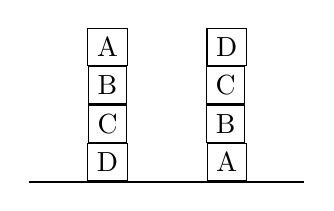
\begin{tikzpicture}[node distance = 0mm, block/.style args = {#1,#2}{fill=#1,text width=#2,shape=square}]
\node (initD) [draw]{D};
\node (initC) [draw, above=of initD.north]{C};
\node (initB) [draw, above=of initC.north]{B};
\node (initA) [draw, above=of initB.north]{A};
\draw[thick] (-1,-0.25) -- (2.5,-0.25);

\node (goalA) [draw, right=10mm of initD]{A};
\node (goalB) [draw, right=10mm of initC]{B};
\node (goalC) [draw, right=10mm of initB]{C};
\node (goalD) [draw, right=10mm of initA]{D};
\end{tikzpicture}
\vspace{0.6cm}
\end{subfigure}%

 \caption{\small Example of a task for learning the STRIPS action model of the blocksworld from a single learning example.}
\label{fig:lexample}
\end{figure}

A solution to a learning task $\Lambda$ is a set of STRIPS operator schema $\Xi$ (with one schema $\xi=\tup{head(\xi),pre(\xi),add(\xi),del(\xi)}$ for each action with a different name in the example plans $\Pi$) that is compliant with the predicates in $\Psi$, the example plans $\Pi$, and their corresponding labels $\Sigma$. 

\subsection{Learning from initial/final states}
Here we reduce the amount of provided input knowledge and define the learning task $\Lambda'=\tup{\Psi,\Sigma}$ that corresponds to watching only the results of the plan executions. In this case no information about the executed plans is given. A solution to the $\Lambda'$ learning task is a set of operator schema $\Xi$ that is compliant only with the predicates in $\Psi$, and the given set of initial and final states $\Sigma$.

In this case, a solution must not only determine a possible STRIPS action model but also the plans that explain the given labels using the learned model (this information about the actions is no longer given in the learning examples). We assume however, that the headers of the operators schema are known. 


\section{Learning STRIPS action models with planning}
Our approach for addressing a learning task $\Lambda$ or $\Lambda'$, is compiling it into a classical planning task with conditional effects $P_{\Lambda}$ or $P_{\Lambda'}$. The intuition behind these compilations is that a solution to the resulting classical planning task is a sequence of actions that:
\begin{enumerate}
\item Programs the STRIPS action model $\Xi$. For each $\xi\in\Xi$, the solution plan determines the literals that belong to its $pre(\xi)$, $del(\xi)$ and $add(\xi)$ sets.
\item Validates the programmed STRIPS action model $\Xi$ using the given input knowledge (the set of labels $\Sigma$, and $\Pi$ if available).  For every label {\small $1\leq t\leq \tau$}, then $\Xi$ is used to produce a final state $s_{n}^t$ starting from the corresponding initial state $s_0^t$. We call this process the validation of the programmed STRIPS action model $\Xi$, at the learning example {\small $1\leq t\leq \tau$}. If information about the corresponding plan $\pi_t\in \Pi$ is available, it is also used in the validation.
\end{enumerate}

Figure~\ref{fig:plan} shows a classical plan for solving a learning task of the $\Lambda$ kind. This classical plan programs and validates the operator schema {\tt\small stack} from the blocksworld, using the plan $\pi_1$ and label $\sigma_1$ shown in Figure~\ref{fig:lexample} (previously specified operator schemes for $pickup$, $putdown$ and $unstack$ are given). In particular the steps $[0,8]$ are the actions for programming the preconditions of the {\tt\small stack} operator, steps $[9,13]$ are the actions for programming the operator effects and steps $[14,22]$ are the actions for validating the programmed operator. The details of the compilation are explained in the remaining of the section.

\begin{figure}[hbt]
\begin{small}
\begin{verbatim}
     0 : (program_pre_clear_stack_v1)
     1 : (program_pre_handempty_stack)
     2 : (program_pre_holding_stack_v2)
     3 : (program_pre_on_stack_v1_v1)
     4 : (program_pre_on_stack_v1_v2)
     5 : (program_pre_on_stack_v2_v1)
     6 : (program_pre_on_stack_v2_v2)
     7 : (program_pre_ontable_stack_v1)
     8 : (program_pre_ontable_stack_v2)
     9 : (program_eff_clear_stack_v1)
    10 : (program_eff_clear_stack_v2)
    11 : (program_eff_handempty_stack)
    12 : (program_eff_holding_stack_v1)
    13 : (program_eff_on_stack_v1_v2)
    14 : (apply_unstack a b i1 i2)
    15 : (apply_putdown a i2 i3)
    16 : (apply_unstack b c i3 i4)
    17 : (apply_stack b a i4 i5)
    18 : (apply_unstack c d i5 i6)
    19 : (apply_stack c b i6 i7)
    20 : (apply_pickup d i7 i8)
    21 : (apply_stack d c i8 i9)
    22 : (validate_1)
\end{verbatim}
\end{small}
 \caption{\small Example of a plan for programing and validating the operator schema $unstack$ using the plan $\pi_1$ and label $\sigma_1$ shown in Figure~\ref{fig:lexample} as well as previously specified operator schemes for $pickup$, $putdown$ and $unstack$.}
\label{fig:plan}
\end{figure}

To formalize our compilations we first define {\small $1\leq t\leq \tau$} classical planning instances $P_t=\tup{F,\emptyset,I_t,G_t}$, one for each leaning example, that belong to the same planning frame (i.e. same fluents and actions and differ only in the initial state and goals). The set of fluents $F$ is built instantiating the predicates in $\Psi$ with the set of different objects appearing in the input learning examples. Formally $\Omega=\{o|o\in \bigcup_{\small 1\leq t\leq \tau} obj(s_0^t)\}$, where $obj$ is a function that returns the set of objects that appear in a fully specified state. The set of actions, $A=\emptyset$, is empty because the action model is initially unknown. Finally, the initial state $I_t$ is given by the state $s_0^t\in \sigma_t$ while goals $G_t$, are defined by the state $s_n^t\in \sigma_t$. 

Now we are ready to formalize our compilations for learning STRIPS action models with classical planning. We start with $\Lambda'$ because it is the learning task that requires the smallest amount of input knowledge. Given a learning task $\Lambda'=\tup{\Psi,\Sigma}$ the compilation outputs a classical planning task $P_{\Lambda'}=\tup{F_{\Lambda'},A_{\Lambda'},I_{\Lambda'},G_{\Lambda'}}$ such that:
\begin{itemize}
\item $F_{\Lambda'}$ extends $F$ with:
\begin{itemize}
\item Fluents representing the programmed action model $pre_f(\xi)$, $del_f(\xi)$ and $add_f(\xi)$, for every $f\in F_v$ and $\xi \in \Xi$). If a fluent $pre_f(\xi)/del_f(\xi)/add_f(\xi)$ holds, it means that $f$ is a precondition/negative effect/positive effect in the STRIPS operator schema $\xi\in \Xi$. 
\item A fluent $mode_{prog}$ indicating whether the operator schemes are being programmed or they are already programmed operators that are being validated. 
\item Fluents $\{test_t\}_{1\leq t\leq \tau}$, indicating the learning example where the programmed action model is being validated.
\end{itemize}
\item $I_{\Lambda'}$, contains the fluents from $F$ that encode $s_0^1$ (the initial state of the first learning example), every $pre_f(\xi)\in F_{\Lambda}$ (our compilation assumes that initially any operator schema contains every possible precondition, no negative effect and no positive effect) and $mode_{prog}$ set to true. 
\item $G_{\Lambda'}=\{test_t\}$, {\small $1\leq t\leq \tau$}, indicates that the programmed action model is validated in all the learning examples.
\item $A_{\Lambda'}$ contains actions of three different kinds:
\begin{enumerate}
\item The actions for programming the an operator schema $\xi\in\Xi$ which includes:
\begin{itemize}
\item The actions for removing a {\em precondition} $f\in F_v$ from the action schema $\xi\in\Xi$. 

\begin{small}
\begin{align*}
\hspace*{7pt}\pre(\mathsf{programPre_{f,\xi}})=&\{\neg del_{f}(\xi),\neg add_{f}(\xi),\\
& pre_{f}(\xi), mode_{prog}\},\\    
\cond(\mathsf{programPre_{f,\xi}})=&\{\emptyset\}\rhd\{\neg pre_{f}(\xi)\}.
\end{align*}
\end{small}

\item The actions for adding a {\em negative} or a {\em positive} effect $f\in F_v$ to the action schema $\xi\in\Xi$.

\begin{small}
\begin{align*}
\hspace*{7pt}\pre(\mathsf{programEff_{f,\xi}})=&\{\neg del_{f}(\xi),\neg add_{f}(\xi),\\                                                   
& mode_{prog}\},\\ 
\cond(\mathsf{programEff_{f,\xi}})=&\{pre_{f}(\xi)\}\rhd\{del_{f}(\xi)\},\\
&\{\neg pre_{f}(\xi)\}\rhd\{add_{f}(\xi)\}.
\end{align*}
\end{small}
\end{itemize}

\item The actions for applying an already programmed operator schema $\xi\in\Xi$ bound with the objects $\omega\subseteq\Omega^{ar(\xi)}$. The binding of the operator schema is done implicitly by order of appearance of the action parameters, i.e. the variables in $pars(\xi)$ are bound to the objects in $\omega$ appearing at the same position. Figure~\ref{fig:compilation} shows the PDDL encoding of the action for applying a programmed operator $stack$.
\begin{small}
\begin{align*}
\hspace*{7pt}\pre(\mathsf{apply_{\xi,\omega}})=&\{pre_{f}(\xi)\implies p(\omega)\}_{\forall p\in\Psi,f=p(pars(\xi))},\\
\cond(\mathsf{apply_{\xi,\omega}})=&\{del_{f}(\xi)\}\rhd\{\neg p(\omega)\}_{\forall p\in\Psi,f=p(pars(\xi))},\\
&\{add_{f}(\xi)\}\rhd\{p(\omega)\}_{\forall p\in\Psi,f=p(pars(\xi))},\\
&\{mode_{prog}\}\rhd\{\neg mode_{prog}\}.
\end{align*}
\end{small}

\item The actions for updating the learning example {\tt\small $1\leq t\leq \tau$} where the programmed action model is validated. 
\begin{small}
\begin{align*}
\hspace*{7pt}\pre(\mathsf{validate_{t}})=&G_t\cup\{test_j\}_{j\in 1\leq j<t}\cup\\
&\cup\{\neg test_j\}_{j\in t\leq j\leq \tau}\cup \{\neg mode_{prog}\},\\
\cond(\mathsf{validate_{t}})=&\{\emptyset\}\rhd\{test_t\}.
\end{align*}
\end{small}
\end{enumerate}
\end{itemize}


\begin{lemma}
Any classical plan $\pi$ that solves $P_{\Lambda'}$ induces an action model $\Xi$ that solves the learning task $\Lambda'$.
\end{lemma}

\begin{proof}[Proof sketch]
The compilation forces that once the preconditions of an operator schema $\Xi$ are programmed, they cannot be altered. The same happens with the positive and negative effects that define an operator schema $\xi \in \Xi$ (besides they can only be programmed after the operator preconditions are programmed). Furthermore, once operator schemes are programmed they can only be applied because of the $mode_{prog}$ fluent. To solve the classical planning task $P_{\Lambda'}$, there is only one way of achieving goals $\{test_t\}$,{\small $1\leq t\leq \tau$}: executing an applicable sequence of programmed operator schemes that reaches the final state $s_n^t$ defined by the associated label $\sigma_t$, starting from $s_0^t$, defined in this same label. If this is achieved for all the input examples of the learning task $\Lambda'$ (i.e. for all the labels $\sigma_t$), it means that the programmed action model $\Xi$ is compliant with the provided input knowledge and hence, it is a solution to $\Lambda'$.
 \end{proof}


\begin{figure}[hbt]
\begin{scriptsize}
\begin{verbatim}
(:action apply_stack
  :parameters (?o1 - object ?o2 - object)
  :precondition
   (and (or (not (pre_on_stack_v1_v1)) (on ?o1 ?o1))
        (or (not (pre_on_stack_v1_v2)) (on ?o1 ?o2))
        (or (not (pre_on_stack_v2_v1)) (on ?o2 ?o1))
        (or (not (pre_on_stack_v2_v2)) (on ?o2 ?o2))
        (or (not (pre_ontable_stack_v1)) (ontable ?o1))
        (or (not (pre_ontable_stack_v2)) (ontable ?o2))
        (or (not (pre_clear_stack_v1)) (clear ?o1))
        (or (not (pre_clear_stack_v2)) (clear ?o2))
        (or (not (pre_holding_stack_v1)) (holding ?o1))
        (or (not (pre_holding_stack_v2)) (holding ?o2))
        (or (not (pre_handempty_stack)) (handempty)))
  :effect
   (and (when (del_on_stack_v1_v1) (not (on ?o1 ?o1)))
        (when (del_on_stack_v1_v2) (not (on ?o1 ?o2)))
        (when (del_on_stack_v2_v1) (not (on ?o2 ?o1)))
        (when (del_on_stack_v2_v2) (not (on ?o2 ?o2)))
        (when (del_ontable_stack_v1) (not (ontable ?o1)))
        (when (del_ontable_stack_v2) (not (ontable ?o2)))
        (when (del_clear_stack_v1) (not (clear ?o1)))
        (when (del_clear_stack_v2) (not (clear ?o2)))
        (when (del_holding_stack_v1) (not (holding ?o1)))
        (when (del_holding_stack_v2) (not (holding ?o2)))
        (when (del_handempty_stack) (not (handempty)))
        (when (add_on_stack_v1_v1) (on ?o1 ?o1))
        (when (add_on_stack_v1_v2) (on ?o1 ?o2))
        (when (add_on_stack_v2_v1) (on ?o2 ?o1))
        (when (add_on_stack_v2_v2) (on ?o2 ?o2))
        (when (add_ontable_stack_v1) (ontable ?o1))
        (when (add_ontable_stack_v2) (ontable ?o2))
        (when (add_clear_stack_v1) (clear ?o1))
        (when (add_clear_stack_v2) (clear ?o2))
        (when (add_holding_stack_v1) (holding ?o1))
        (when (add_holding_stack_v2) (holding ?o2))
        (when (add_handempty_stack) (handempty))
        (when (modeProg) (not (modeProg)))))
\end{verbatim}
\end{scriptsize}
 \caption{\small Action for applying an already programmed operator schema $stack$ as encoded in PDDL.}
\label{fig:compilation}
\end{figure}


\section{Constraining the learning hypothesis space with additional input knowledge}
Here we show that further input knowledge can be used to reduce the space of the possible action models and make the learning of STRIPS action models more practicable. 

\subsection{Static predicates}
A {\em static predicate} $p \in \Psi$ is a predicate that does not appear in the effects of any action schema $\xi\in\Xi$. Therefore, one can get rid of the mechanism for programming static predicates as action effects. Formally, given a static predicate $p$:
\begin{itemize}
\item The fluents $del_f(\xi)$ and $add_f(\xi)$, such that $f\in F_v$ is an instantiation of the static predicate $p$ in $\Omega_V$, can be removed from the compilation for every $\xi\in\Xi$.
\item The actions $\mathsf{programEff_{f,\xi}}$ (s.t. $f\in F_v$ is an instantiation of the static predicate $p$ in $\Omega_V$) can also be removed from the compilation.
\end{itemize}

Furthermore, certain fluents and actions can also be removed if a precondition $f\in F_v$ is not possible for the schema $\xi\in\Xi$ according to a given example {\small $1\leq t\leq \tau$}. For instance in the {\em zenotravel} domain fluents $pre\_next\_board\_v1\_v1$, $pre\_next\_debark\_v1\_v1$, $pre\_next\_fly\_v1\_v1$, $pre\_next\_zoom\_v1\_v1$, $pre\_next\_refuel\_v1\_v1$ that indicates that a precondition {\tt\small(next ?v1 ?v2 - flevel)} is programmed can be discarded (and their corresponding programmming actions) because there is no state in the labels $\Sigma$ that can satisfy them.

In our evaluation section we shown how to compute candidates of static predicates from the inputs to our learning tasks and how using this knowledge affects to the performance of our approach. 

\subsection{Previously specified action models}
Our compilation does not require to start the learning of STRIPS action models from scratch and accepts partially specified operator schema where some preconditions are effects are a priori known.

The known preconditions and effects are encoded as fluents $pre_f(\xi)$, $del_f(\xi)$ and $add_f(\xi)$ set to true that are part of the initial state $I_{\Lambda'}$. The corresponding programming actions ($\mathsf{programPre_{f,\xi}}$ and $\mathsf{programEff_{f,\xi}}$) are removed from $A_{\Lambda'}$ reducing the number of applicable actions  and making the classical planning task $P_{\Lambda'}$ easier to be solved. With this regard, the classical plan of Figure~\ref{fig:plan} is a solution to a learning task for getting the blocksworld action model where the operator schema for {\tt\small pickup}, {\tt\small putdown} and {\tt\small unstack} are known in advance. 

In the extreme, the compilation can also be used to validate whether an observed plan follows a given STRIPS action model. In this case the action model to validate is coded in the initial state $I_{\Lambda'}$, any programmed action is removed from $A_{\Lambda'}$ and the $mode_{prog}$ fluent is set to false. If a solution plan is found to $P_{\Lambda'}$ it means that the given STRIPS action model is {\em valid} for the given examples. If $P_{\Lambda'}$ is unsolvable it means that the given STRIPS action model is invalid since it cannot satisfy the given examples. Tools for plan validation like VAL~\cite{howey2004val} can also be used at this point but note that the compilation approach does not require a plan so the validation of an STRIPS action model can be done with just an initial and a final state.

\subsection{Example plans}
Here  we extend our compilation to address the learning scenario defined by the $\Lambda$ task where, a set of plans $\Pi$ is available so it is used to reduce the space of possible action models. Given a learning task $\Lambda=\tup{\Psi,\Pi,\Sigma}$, the compilation outputs a classical planning task $P_{\Lambda}=\tup{F_{\Lambda},A_{\Lambda},I_{\Lambda},G_{\Lambda}}$ that extends $P_{\Lambda}'$ as follows: 
\begin{itemize}
\item $F_{\Lambda}$ extends $F_{\Lambda'}$ by including also the fluents $F_{\Pi}=\{plan(name(\xi),j,\Omega^{ar(\xi)})\}$ to code the $j$ steps of a plan in $\Pi$, with $F_{\Pi_t}\subseteq F_{\Pi}$ encoding $\pi_t\in \Pi$. We denote $\pi_t$ a solution plan to a classical planning instance $P_t$. In addition fluents $at_j$ and $next_{j,j_2}$, {\small $1\leq j<j2\leq n$}, are also added to represent the plan steps where the programmed action model is validated.
\item $I_{\Lambda}$ is extended with the fluents from $F_{\Pi_1}$ that encode the plan $\pi_1\in \Pi$ for solving $P_1$, and the fluents $at_1$ and $\{next_{j,j_2}\}$, {\small $1\leq j<j2\leq n$}, for indicating where to start validating the programmed action model. Goals are the same as in the previous compilation $G_{\Lambda}=G_{\Lambda}'$ so again require that the programmed action model is validated in all  the learning examples.
\item With respect to $A_{\Lambda}$.
\begin{enumerate}
\item The actions for programming the preconditions/effects of a given operator schema $\xi\in\Xi$ are the same.
\item The actions for applying an operator have an extra precondition $f\in F_{\Pi_t}$ that encodes the current plan step and extra conditional effects $\{at_{j}\}\rhd\{\neg at_{j},at_{j+1}\}_{\forall j\in [1,n]}$ for advancing the plan step.
\item The actions for updating the active test have an extra precondition, $at_{|\Pi_t|}$, to indicate that the current plan $\Pi_t$ was fully executed and extra conditional effects to load the next plan $\Pi_{t+1}$:
\begin{small}
\begin{align*}
&\{f\}\rhd\{\neg f\}_{f\in F_{\Pi_t}}, \{\emptyset\}\rhd\{f\}_{f\in F_{\Pi_t+1}},\{\emptyset\}\rhd\{\neg at_{|\pi_t|},at_1\}.
\end{align*}
\end{small}
\end{enumerate}
\end{itemize}


\section{Evaluation}
We evaluated our approach for learning STRIPS action models from different amounts of available input knowledge.

\subsection{Setup}
All the experiments run on an Intel Core i5 3.10 GHz x 4 with 4 GB of RAM. The domains used in the evaluation are IPC domains that satisfy the STRIPS requirement~\cite{fox2003pddl2}, and are taken from the {\sc planning.domains} repository~\cite{muise2016planning}.

\subsubsection{The classical planner.}
The classical planner used to solve the instances that result from our compilations is the SAT-based classical planner {\sc Madagascar}~\cite{rintanen2014madagascar}. We decided to use a SAT-based planner because its ability to deal with planning instances populated with dead-ends. In addition, in a SAT-based classical planner all the actions for programming the STRIPS actions preconditions can be done in parallel, in a single planning step, because they do not interact reducing significantly the planning horizon. Likewise, all the actions for programming an action effect can also be applied in a single planning step.  


\subsubsection{The evaluation metrics.}
The quality of the learned models is quantified with the {\em precision} and {\em recall} metrics. These two metrics are frequently used in pattern recognition, information retrieval and binary classification and are more informative that simply counting the number of model errors or computing the {\em symmetric difference} between the learned model and the baseline ~\cite{davis2006relationship}.

Intuitively precision gives a notion of {\em soundness} while recall gives a notion of the {\em completeness} of the learned models. Formally $Precision=\frac{tp}{tp+fp}$, where $tp$ is the number of true positives (predicates that correctly appear in the action model) and $fp$ is the number of false positives (predicates appear in the learned action model that should not appear). On the other hand recall is formally defined as $Recall=\frac{tp}{tp+fn}$ where $fn$ is the number of false negatives (predicates that should appear in the learned action model but are missing). 


\subsubsection{The learning examples.}


\subsection{Learning action models from example plans}
Here we assess the performance of our learning approach when addressing $\Lambda$ learning tasks. Here the {\em precision} and {\em recall} metrics are computed in the learned models with respect to the actual models taken as reference. Table~\ref{tab:results_plans} summarizes the obtained results, precision ({\bf P}) and recall ({\bf R}) is computed separately for the preconditions ({\bf Pre}), positive effects ({\bf Add}) and negative Effects ({\bf Del}). 

\begin{table}[hbt!]
	\begin{small}
	\begin{center}
		\begin{tabular}{l|l|l|l|l|l|l|}
			 & \multicolumn{2}{|c|}{\bf Pre} & \multicolumn{2}{|c|}{\bf Add} & \multicolumn{2}{|c|}{\bf Del}  \\ \cline{2-7}			 
			  & \multicolumn{1}{|c|}{\bf P} & \multicolumn{1}{|c|}{\bf R} & \multicolumn{1}{|c|}{\bf P} & \multicolumn{1}{|c|}{\bf R} & \multicolumn{1}{|c|}{\bf P} & \multicolumn{1}{|c|}{\bf R} \\
			\hline
			Blocks & 1.0 & 1.0 & 1.0 & 1.0 & 1.0 & 1.0 \\
			Driverlog & 1.0 & 0.4 & 0.6 & 0.8 & 1.0 & 0.8 \\
			Ferry & 0.8 & 0.5 & 1.0 & 1.0 & 1.0 & 1.0 \\
			Floortile & 0.5 & 0.6 & 0.9 & 0.8 & 1.0 & 0.9 \\
			Gripper & 1.0 & 0.6 & 1.0 & 1.0 & 1.0 & 1.0 \\
			Miconic & 0.7 & 0.3 & 1.0 & 0.7 & 0.7 & 1.0 \\
			Satellite & 0.6 & 0.2 & 1.0 & 1.0 & 1.0 & 0.75 \\
			Transport & 1.0 & 0.3 & 0.5 & 0.8 & 1.0 & 0.6 \\
			Visitall & 1.0 & 0.5 & 1.0 & 1.0 & 1.0 & 1.0 \\
			Zenotravel & 1.0 & 0.3 & 0.7 & 0.8 & 1.0 & 0.7
		\end{tabular}
	\end{center}
	\end{small}
\caption{\small The {\em precision} and {\em recall} values achieved by the learned models in the $\Lambda$ learning tasks.}
\label{tab:results_plans}
\end{table}

Table~\ref{tab:time_plans} reports the total planning time, and the preprocessing time (in seconds) invested by the classical planner {\sc Madagascar} to solve the classical planning tasks that result from our compilation as well as the plan length of the found solutions. 	

\begin{table}[hbt!]
\begin{small}
	\begin{center}
		\begin{tabular}{l|c|c|c|}			 
			Domain & Total time & Preprocess & Plan length  \\
			\hline
			Blocks & 0.04 & 0.00 & 72 \\
			Driverlog & 0.10 & 0.06 & 127 \\
			Ferry & 0.20 & 0.10 & 58 \\
			Floortile & 2.15 & 1.21 & 170 \\
			Gripper & 0.01 & 0.00 & 45 \\
			Miconic & 0.10 & 0.09 & 54 \\
			Satellite & 0.20 & 0.14 & 67 \\
			Transport & 0.20 & 0.18 & 60 \\
			Visitall & 0.43 & 0.39 & 37 \\
			Zenotravel & 2.78 & 2.76 & 70			
		\end{tabular}
	\end{center}
        \end{small}
	\caption{\small Planning time, preprocessing time and Plan length.}
	\label{tab:time_plans}	
\end{table}

\subsection{Exploiting static predicates}
Here we repeat the previous evaluation but compute now a candidates of static predicates from the inputs to the learning task and exploit this knowledge (as explained in Section~\ref{}) to reduce the space of possible action models. The set of considered candidate {\em static predicates} is the set of predicates whose instantiation appear the same in the initial and final states for all the learning examples {\small $1\leq t\leq \tau$}. Tables~\ref{tab:results_plans_static} and~\ref{tab:time_plans_static} show the obtained results.	

\begin{table}[hbt!]
\begin{small}
	\begin{center}
		\begin{tabular}{l|l|l|l|l|l|l|}
			 & \multicolumn{2}{|c|}{\bf Pre} & \multicolumn{2}{|c|}{\bf Add} & \multicolumn{2}{|c|}{\bf Del}  \\ \cline{2-7}			 
			  & \multicolumn{1}{|c|}{\bf P} & \multicolumn{1}{|c|}{\bf R} & \multicolumn{1}{|c|}{\bf P} & \multicolumn{1}{|c|}{\bf R} & \multicolumn{1}{|c|}{\bf P} & \multicolumn{1}{|c|}{\bf R} \\
			\hline 
		\end{tabular}
	\end{center}
	\end{small}
\caption{\small The {\em precision} and {\em recall} values achieved by the learned models in the $\Lambda$ learning tasks exploiting the computed static predicates.}
\label{tab:results_plans_static}
\end{table}


\begin{table}[hbt!]
\begin{small}
	\begin{center}
		\begin{tabular}{l|c|c|c|}			 
			Domain & Total time & Preprocess & Plan length  \\
			\hline 			
		\end{tabular}
	\end{center}
        \end{small}
	\caption{\small Planning time, preprocessing time and Plan length exploiting the computed static predicates.}
	\label{tab:time_plans_static}	
\end{table}

\subsection{Learning from partially specified action models}

Here we evaluate the ability of the compilation to support partially specified action models. In this case instead of learning the action models from scratch the model of half of the actions is given as input of the learning task. Tables~\ref{tab:results_plans_partial} and~\ref{tab:time_plans_partial} summarizes the obtained results.	

\begin{table}[hbt!]
\begin{small}
	\begin{center}
		\begin{tabular}{l|l|l|l|l|l|l|}
			 & \multicolumn{2}{|c|}{\bf Pre} & \multicolumn{2}{|c|}{\bf Add} & \multicolumn{2}{|c|}{\bf Del}  \\ \cline{2-7}			 
			  & \multicolumn{1}{|c|}{\bf P} & \multicolumn{1}{|c|}{\bf R} & \multicolumn{1}{|c|}{\bf P} & \multicolumn{1}{|c|}{\bf R} & \multicolumn{1}{|c|}{\bf P} & \multicolumn{1}{|c|}{\bf R} \\
			\hline
			Blocks & 1.0 & 1.0 & 1.0 & 1.0 & 1.0 & 1.0 \\
			Driverlog & 1.0 & 0.4 & 1.0 & 1.0 & 1.0 & 0.7 \\
			Ferry & 1.0 & 0.6 & 0.5 & 1.0 & 1.0 & 1.0 \\
			Floortile & 0.5 & 0.6 & 1.0 & 0.8 & 1.0 & 0.8 \\
			Gripper & 1.0 & 0.5 & 1.0 & 1.0 & 1.0 & 1.0 \\
			Miconic & 1.0 & 0.2 & 1.0 & 1.0 & 1.0 & 1.0 \\
			Satellite & 1.0 & 0.5 & 0.5 & 1.0 & 1.0 & 1.0 \\
			Transport & 1.0 & 0.2 & 1.0 & 1.0 & 1.0 & 0.5 \\
			Zenotravel & 1.0 & 0.5 & 0.6 & 0.6 & 1.0 & 1.0                         
		\end{tabular}
	\end{center}
	\end{small}
\caption{\small The {\em precision} and {\em recall} values achieved by the learned models in the different domains.}
\label{tab:results_plans_partial}
\end{table}

\begin{table}[hbt!]
\begin{small}
	\begin{center}
		\begin{tabular}{l|c|c|c|}			 
			Domain & Total time & Preprocess & Plan length  \\
			\hline
			Blocks & 0.07 & 0.01 & 54  \\
			Driverlog & 0.06 & 0.03 & 71 \\
			Ferry & 0.18 & 0.14 & 50 \\
			Floortile & 0.81 & 0.68 & 92 \\
			Gripper & 0.01 & 0.00 & 37 \\
			Miconic & 0.06 & 0.04 & 40  \\
			Satellite & 0.18 & 0.12 & 43 \\
			Transport & 0.15 & 0.14 & 33 \\
			Zenotravel & 2.54 & 2.54 & 42                         
		\end{tabular}
	\end{center}
        \end{small}
	\caption{\small Planning time, preprocessing time and Plan length.}
	\label{tab:time_plans_partial}	
\end{table}



\subsection{Validating action models with classical planning}
Here we evaluate the performance of the compilation to validate whether a given action mode is compliant with a given set of observations. Table~\ref{tab:time_plans_val} reports the planning time, and prepossessing time used to solve the classical planning task that results from our compilation as well as the plan length of the found solutions.
\begin{table}[hbt!]
\begin{small}
	\begin{center}
		\begin{tabular}{l|c|c|r|}			 
			Domain & Total time & Preprocess & Plan length  \\
			\hline
			Blocks & 0.00 & 0.00 \\
			Driverlog & 0.04 & 0.04 \\
			Ferry & 0.01 & 0.01 \\
			Floortile & 0.03 & 0.03 \\
			Gripper & 0.00 & 0.00 \\
			Miconic & 0.01 & 0.01 \\
			Satellite & 0.30 & 0.29 \\
			Transport & 0.02 & 0.02 \\
			Visitall & 0.07 & 0.07  \\
			Zenotravel & 11.65 & 11.39 			
		\end{tabular}
	\end{center}
        \end{small}
	\caption{\small Planning time, preprocessing time and Plan length for validating a given action model.}
	\label{tab:time_plans_val}	
\end{table}


\subsection{Learning action models from example states}
When the set of input planning task is not available, the planner determines also the actions that must satisfying the input labels so actions can reformulated and still be compliant with the learning examples. For instance a blocksworld can be learned where the operator {\small\tt stack} is defined with the preconditions and effects of the {\small\tt unstack} operator and vice versa. 

\subsubsection{Learning exploiting static predicates}
\subsubsection{Learning from partially specified action models}





\section{Related work}

The  LIVE  system  (Shen  and  Simon,  1989)  was  an  extension  of  the  General  Problem  Solver  (GPS) framework (Ernst and Newell, 1969) with a learning component. LIVE alternated problem solving with model  learning  to  automatically  define  operators.  The  decision  about  when  to  alternate  depended  onsurprises,  that  is  situations  where  an  action  effects  violated  its  predicted  model.  EXPO  (Gil,  1992) generated plans with the  PRODIGY  system (Minton, 1988), monitored the plans execution, detected differences in the predicted and the observed states and constructed a set of specific hypotheses to fix those differences. Then the  EXPO  filtered the hypotheses heuristically.  OBSERVER  (Wang, 1994) learned operators by monitoring expert agents and applying the version spaces algorithm (Mitchell, 1997) to the observations. When the system already had an operator representation, the preconditions were updated by removing facts that were not present in the new observation’s pre-state; the effects were augmented by adding facts that were in the observation’s delta-state. All of these early works were based on direct liftings of the observed states. They also benefit from experience beyond simple interaction with the environment such as exploratory plans or external teachers, but  none  provided  a  theoretical  justification  for  this  second  source  of  knowledge.  The  work  recently reported in (Walsh and Littman, 2008) succeeds in bounding the number of interactions the learner must complete to learn the preconditions and effects of a STRIPS action model. This work shows that learning STRIPS  operators  from  pure  interaction  with  the  environment,  can  require  an  exponential  number  of samples, but that limiting the size of the precondition lists enable sample-efficient learning (polynomial in the number of actions and predicates of the domain). The work also proves that efficient learning is also possible without this limit if an agent has access to an external teacher that can provide solution traces on demand.

Others systems have tried to learn more expressive action models for deterministic planning in fully observable environments. Examples would include the learning of conditional costs for AP actions (Jess Lanchas and Borrajo, 2007) or the learning of conditional effects with quantifiers (Zhuo et al., 2008).

In addition action model learning has been studied in domains where there is partial state observability. ARMS uses the same kind od learning examples but assumes the exampls are given and proceeds in two phases. In the first phase, ARMS extracts frequent action sets from plans that share a common set of parameters. ARMS also finds some frequent literal-action pairs with the help of the initial state and the goal state that provide an initial guess on the actions preconditions, and effects. In the second phase, ARMS uses the frequent action sets and literal-action pairs to define a set of weighted constraints that must hold in order to make the plans correct. Then, ARMS solves the resulting weighted MAX-SAT problem and produces action models from the solution of the SAT problem. This process iterates until all actions are modelled. For a complex planning domain that involves hundreds of literals and actions, the corresponding weighted MAX-SAT representation is likely to be too large to be solved efficiently as the number of clauses can reach up to tens of thousands. For that reason ARMS implements a hill-climbing method that models the actions approximately. Consequently, the ARMS output is a model which may be inconsistent with the examples.

(Amir and Chang, 2008) introduced an algorithm that tractably generates all the STRIPS-like models that  could  have  lead  to  a  set  of  observations.  Given  a  formula  representing  the  initial  belief  state,  a sequence of executed actions and the corresponding observed states(where partial observations of states are given), it builds a complete explanation of observations by models of actions through a Conjunctive Normal Form (CNF) formula. By linking the possible states of fluents to the effect propositions in the action models, the complexity of the CNF encoding can be controlled to find  exact  solutions  efficiently  in  some  circumstances.  The  learning  algorithm  updates  the  formula  of the belief state with every action and observation in the sequence. This update makes sure that the new formula represents all the transition relations consistent with the actions and observations. The formula returned at the end includes all consistent models, which can then be retrieved with additional processing. Unlike the previous approaches, the one described in (Mour ao et al., 2008) deals with both missing and noisy predicates in the observations. For each action in a given domain, they use kernel perceptrons to learn predictions of the domain properties that change because of the action execution. LOCM (Cresswellet al., 2009) induces action schemas without being provided with any information about initial, goal or intermediate state descriptions for the example action sequences. LOCM receives descriptions of plans or plan fragments, uses them to create states machines for the different domain objects and extracts the action schemas from these state machines.

~\cite{stern2017efficient}.


\section{Conclusions}
The paper presented a novel approach for learning STRIPS action models from examples exclusively using classical planning. Interestingly the approach is flexible to different amounts of available input knowledge and accepts partially specified action models.   

The empirical evaluation shows that, when example plans are available, our approach can compute accurate action models. When action plans are not available our approach is still able to produce action models compliant with the input information. In this case, since learning is not constrained by actions it can change the semantics of the operators. An interesting research direction related to this issue is {\em domain reformulation} to use actions in a more efficient way, reduce the set of actions identifying dispensable information or exploitin features that allow more compact solutions like the {\em reachable} or {\em movable} features in the Sokoban domain. 

With regard to efficiency, the size of the compiled classical planning instances depend on the number of input examples. On the other hand the empirical results show that our approach, since is based on inferences instead of statistics, is able to generate non-trivial models from very small data sets.

As far as we know, this is the first work on learning action models using a classical planner, which opens the door to the bootstrapping of action model. That is that a planner collects by its own the data necessary learn an action model for a given planning task. With this regard, collecting {\em informative} examples for learning planning action models is challenging open issue. Planning actions include preconditions that are only satisfied by specific sequences of actions, and often, with a low probability of being chosen by chance~\cite{fern2004learning}. The recent success of recent algorithms for exploring planning tasks~\cite{geffner:novelty:IJCAI17} motivates the development of novel approaches that do not assume that a learning set of plans is given apriori but instead, autonomously collect the learning examples.


\subsection*{Acknowledgment}
\begin{small}
Diego Aineto is partially supported by the {\it FPU} program funded by the Spanish government. Sergio Jim\'enez is partially supported by the {\it Ramon y Cajal} program funded by the Spanish government.
\end{small}

\newpage

\bibliographystyle{aaai}
\bibliography{strips-learning}
\end{document}
